\documentclass{report}

% Packages
\usepackage{import}
\usepackage{xcolor}
\usepackage{cancel}
\usepackage{mathtools}
\usepackage{hyperref}
\usepackage{setspace}
\usepackage{float}
\usepackage{parskip}
\setlength{\parindent}{0pt}
\usepackage{scalerel}

\renewcommand{\vec}{\mathbf}
\DeclareMathOperator{\vectorprojection}{proj}
\NewDocumentCommand{\proj}{s e{_} m}{%
    \IfBooleanTF{#1}{#3_{\stretchrel*{\parallel}{\perp}#2}}{\vectorprojection_{#2}#3}
}
\renewcommand{\Re}{\operatorname{Re}}
\renewcommand{\Im}{\operatorname{Im}}
\renewcommand{\Arg}{\operatorname{Arg}}
\renewcommand{\arcsec}{\operatorname{sec}^{-1}}

% Custom perms and combs commands
\newcommand\Myperm[2][^n]{\prescript{#1\mkern-2.5mu}{}P_{#2}}
\newcommand\Mycomb[2]{\prescript{#1\mkern-0.5mu}{}C_{#2}}
% Custom column vector command
\newcommand{\cvec}[1]{ \begin{pmatrix} #1 \end{pmatrix} }
% Custom determinant command
\newcommand{\det}[1]{ \begin{vmatrix} #1 \end{vmatrix} }

% Colors
\definecolor{yorhabg}{HTML}{131314}
\definecolor{yorhafg}{HTML}{C9C7CD}
\definecolor{yorhagrid}{HTML}{B5AF9C}
\definecolor{mred}{HTML}{D67069}
\definecolor{mblue}{HTML}{6887A1}

\usepackage[dvipsnames]{xcolor}
\definecolor{pastel_red}{RGB}{255, 173, 173}
\definecolor{pastel_orange}{RGB}{255, 214, 165}
\definecolor{pastel_yellow}{RGB}{253, 255, 182}
\definecolor{pastel_green}{RGB}{176, 217, 176}
\definecolor{pastel_blue}{RGB}{167, 199, 231}
\definecolor{pastel_purple}{RGB}{222, 218, 244}

\pagecolor{yorhabg}		% Set background color
\color{yorhafg}

\import{preamble.sty}

\usepackage[T1]{fontenc}			% Font package

\usepackage{fouriernc}

\usepackage{sectsty}
\usepackage{graphicx}
\usepackage{amsmath}
\usepackage{amsfonts}
\usepackage{amssymb}
\usepackage[skins, most]{tcolorbox}

\DeclareMathOperator{\sgn}{sgn}

\DeclareMathOperator{\area}{area}
\DeclareMathOperator{\sech}{sech}
\DeclareMathOperator{\cosech}{cosech}
\usepackage{tikz}
\usepackage{eso-pic}
\usetikzlibrary{calc, shadows.blur}
\usetikzlibrary{angles, quotes}
\usetikzlibrary{3d}

% Margins
\topmargin=0in
\evensidemargin=0in
\oddsidemargin=0in
\textwidth=6.5in
\textheight=9.0in
\headsep=0.25in

\AtBeginEnvironment{tcolorbox}{\small}

\newtcolorbox{imp}{enhanced,arc=0mm,colback=yorhabg,colframe=mred,leftrule=10mm,coltext=yorhafg,%
overlay={\node[anchor=west,outer sep=2pt] at (frame.west) {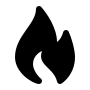
\includegraphics[width=6mm]{images/imageb.png}}; }}

\newtcolorbox{shortcut}{enhanced,arc=0mm,colback=yorhabg,colframe=mred,leftrule=10mm,coltext=yorhafg, coltitle=yorhabg, title=\texttt{Shortcut.}, 
overlay={\node[anchor=west,outer sep=2pt] at (frame.west) {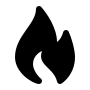
\includegraphics[width=6mm]{images/imageb.png}}; }}

\newtcolorbox{question}[1]{
    enhanced, 
    colback=yorhabg,
    colframe=mblue,
    coltext=yorhafg,
    coltitle=yorhabg,
    attach boxed title to top left={yshift*=-\tcboxedtitleheight}, 
    title=\texttt{#1},
    boxed title size=title,
    boxed title style={%
        rounded corners=northeast, 
        rounded corners=northwest, 
        colback=tcbcolframe, 
        boxrule=0pt,
    },
    underlay boxed title={%
        \path[fill=tcbcolframe] (title.south west)-- (title.south east) 
            to[out=0, in=180] ([xshift=5mm]title.east)--
            (title.center-|frame.east)
            [rounded corners=5pt] |- 
            (frame.north) -| cycle; 
    },
}

\newcommand\bb[1]{\textcolor{yorhafg}{\textbf{#1}}}

% Spacing
\setlength{\jot}{1.5em}
\setlength{\thickmuskip}{10}
\setlength{\medmuskip}{7}
\setlength{\thinmuskip}{5}
\setstretch{1.25}

\title{\textbf{MATH1141: Higher Mathematics 1B (Algebra)}}
\author{L. Cheung}
\date{\today}

\begin{document}

\maketitle
\tableofcontents
\newpage

\chapter{Functions of several variables}

	\section{Motivations, sketching surface, and partial derivatives}

		\subsection{Function of two variables}

			We will consider functions of the type
				\begin{align*}
					z = F(x,y), \quad (x,y) \in D
				\end{align*}
			where $D \subseteq \mathbb{R}^2$ is the domain of $F$ and $F$ is real-valued. We write $F: D \subseteq \mathbb{R}^2 \to \mathbb{R}$.

			For example:
			\begin{itemize}
				\item $F(x,y) = 2x + y^6$ and $D = \mathbb{R}^2$
				\item $F(x,y) = xe^y$ and $D = \mathbb{R}^2$
			\end{itemize}

			\textcolor{pastel_yellow}{Note}: if $D = \mathbb{R}^2$, sometimes the domain is not explicitly written.

			\subsubsection{Geometric representation}

				The function of one variable: $y = f(x), \; x \in [a,b]$ can be represented as a curve in $\mathbb{R}^2$.

				Similarly, a function of two variables: $z = F(x,y), \; (x,y) \in D$ can be described as a surface in $\mathbb{R}^3$

		\subsection{Sketching and visualising surfaces}

			Consider a surface defined by 
				\begin{align*}
					z = F(x,y).
				\end{align*}

			Conventionally, $z$ is the distance above or below the $x,y$-plane.

			A \textbf{level curve} of a function, $F:\mathbb{R}^2 \to \mathbb{R}$, is a curve in $\mathbb{R}^2$ defined by $F(x,y) = C$, where $C$ is a constant. This can be visualised by cutting a surface with a plane. Typically this plane is parallel to the $xy$-plane

			\begin{question}{Example}
				Sketch the surface defined by
					\begin{align*}
						z = F(x,y) = x^2 + y^2
					\end{align*}

				\begin{enumerate}
					\item Sketch some level curves for different values $C$.
						\begin{itemize}
							\item Set $z = C = 0 \Rightarrow \; x^2 + y^2 = 0 \Rightarrow$ Singular point at origin
							\item Set $z = C = 1 \Rightarrow \; x^2 + y^2 = 1 \Rightarrow$ Circle centred at 0 with radius $1$
							\item Set $z = C = 4 \Rightarrow \; x^2 + y^2 = 4 \Rightarrow$ Circle centred at 0 with radius $2$
							\item Set $z = C = 8 \Rightarrow \; x^2 + y^2 = 8 \Rightarrow$ Circle centred at 0 with radius $2 \sqrt{2}$
						\end{itemize}
					\item Sketch the curves of intersection between the surface $z = x^2 + y^2$ and the $yz$-plane (set $x = 0$) or $xz$-plane (set $y = 0$).
						\begin{itemize}
							\item In this example, both the intersections form parabolas.
						\end{itemize}
				\end{enumerate}
			\end{question}

			\begin{question}{Example}
				Sketch the surface defined by $x^2 + y^2 - z^2 = 1$.

				\begin{enumerate}
					\item Level curves
						\begin{itemize}
							\item level curves with $z = 0$ is a circle with radius 1
							\item level curves with $z = \pm 1$ are circles with radius $\sqrt{2}$
							\item level curves with $z = \pm 2$ are circles with radius $\sqrt{5}$
						\end{itemize}
					\item Intersections between the surface and the $yz$-plane gives $y^2 - z^2 = 1$.
					\item These pieces of information can be put together to form the surface
				\end{enumerate}
				
			\end{question}

		\subsection{Partial differentiation}

			Informally: differentiate with respect to one of the variables by holding the other variable fixed.

			\begin{question}{Definition}
				If $F: \mathbb{R}^2 \to \mathbb{R}$ is a function of two variables $x$ and $y$, then the partial derivatives of $F(x,y)$ with respect to $x$ and $y$ at the point $(x_0, y_0)$ are defined by
					\begin{align*}
						\frac{\partial F}{\partial x} (x_0, y_0) = \lim_{h\to 0} \frac{F(x_0 + h, y_0) - F(x_0, y_0)}{h},
					\end{align*}
				and
					\begin{align*}
						\frac{\partial F}{\partial y} (x_0, y_0) = \lim_{h\to 0} \frac{F(x_0, y_0 + h) - F(x_0, y_0)}{h},
					\end{align*}
				wherever these limits exist.
			\end{question}

			If a function $F$ has partial derivatives with respect to $x$ and $y$, then:
				\begin{itemize}
					\item The partial derivative with respect to $x$ may be denoted by
						\begin{align*}
							\frac{\partial F}{\partial x} \equiv F_x \equiv D_1F.
						\end{align*}
					\item The partial derivative with respect to $y$ may be denoted by
						\begin{align*}
							\frac{\partial F}{\partial y} \equiv F_y \equiv D_2F.
						\end{align*}
				\end{itemize}

			The rules for partial derivatives are similar to that of normal derivatives.

			\begin{question}{Example}
				Consider
					\begin{align*}
						F(x,y) = e^{y^2} \cos(x^2y) + e^{x^2y} \sin(y).
					\end{align*}
				Compute the partial derivatives of $\frac{\partial F}{\partial x}$ and $\frac{\partial F}{\partial y}$.
				\begin{align*}
					\frac{\partial F}{\partial x} &= \frac{\partial}{\partial x} \left[e^{y^2} \cos(x^2y)\right] + \frac{\partial}{\partial x} \left[x^{y^2} \sin(y)\right]	\\
												  &= e^{y^2} \left[-\sin(x^2y) (2xy)\right] + \sin(y) e^{y^2}(2xy)
				\end{align*}
			\end{question}

		\subsection{Geometrical Interpretation}

			Recall that $\frac{\partial F}{\partial x} (x_0, y_0) = \displaystyle\lim_{h\to 0} \frac{F(x_0 + h, y_0) - F(x_0,y_0)}{h}$.

			$\frac{\partial F}{\partial x} (x_0,y_0)$ is the slope of the tangent to the cross section at $(x_0,y_0)$ when the surface $z = F(x,y)$ is intersected with the plane $y = y_0$.

			This can be applied similarly to the derivative $\frac{\partial F}{\partial y}$

		\subsection{Second Order Partial Derivatives}

			A second order partial derivative is a partial derivative of a first order partial derivative.
				\begin{align*}
					\frac{\partial^2 F}{\partial x} \equiv \frac{\partial}{\partial x} (\frac{\partial F}{\partial x}) \equiv F_{xx} \equiv D_1D_1F	\\
					\frac{\partial^2 F}{\partial y} \equiv \frac{\partial}{\partial y} (\frac{\partial F}{\partial y}) \equiv F_{yy} \equiv D_2D_2F	\\
					\frac{\partial^2 F}{\partial x \partial y} \equiv \frac{\partial}{\partial x} (\frac{\partial F}{\partial y}) \equiv F_{yx} \equiv D_1D_2F	\\
					\frac{\partial^2 F}{\partial y \partial x} \equiv \frac{\partial}{\partial y} (\frac{\partial F}{\partial x}) \equiv F_{xy} \equiv D_2D_1F	\\
				\end{align*}

			\begin{question}{The Mixed Derivative Theorem}
				Suppose that $F$ is a function of two variables. If $F$ and all its first and second order partial derivatives are continuous, then
					\begin{align*}
						\frac{\partial^2 F}{\partial x \partial y} = \frac{\partial^2 F}{\partial y \partial x}
					\end{align*}
			\end{question}

			\begin{question}{Definition}
				Consider a function $G$ on $\mathbb{R}^2$ with variables $x$ and $y$. The function $G$ is continuous at the point $(x_0,y_0) \in \mathbb{R}^2$ if
					\begin{align*}
						\lim_{\substack{x \to x_0 \\ y \to y_0}} G (x,y) = F(x_0,y_0).
					\end{align*}
			\end{question}

			\begin{itemize}
				\item Finite sums/products of continuous functions are continuous, and compositions of continuous functions are continuous
				\item The mixed derivative theorem tells us that for a function which can be written as a finite sum/product of a polynomials, sine, cosine, exponential functions, all derivatives of all orders are continuous, and so we get the equality of all mixed derivatives.
				\item The existence of partial derivatives at a point does not imply continuity at a point
			\end{itemize}

			\begin{question}{Example}
				Consider the function
					\begin{align*}
						F(x,y) = \begin{cases} \frac{xy}{x^2 + y^2} &\text{for }(x,y)\neq (0,0) \\ 0 &\text{for } (x,y) = (0,0)\end{cases}.
					\end{align*}
				We see that $\frac{\partial F}{\partial x} (0,0) = \frac{\partial F}{\partial y} (0,0) = 0$, but $F(x,y)$ is not continuous at $(0,0)$.
			\end{question}

\chapter{Tangent planes, normal vectors, and error estimation}

	\section{Tangent Lines and Normals}

		Suppose that $(x_0,y_0)$ is a point that lies on the curve $y = f(x)$. If the curve has a tangent line at $(x_0,y_0)$:
		\begin{itemize}
			\item The tangent line has the equation
				\begin{align*}
					y = y_0 + f'(x_0)(x - x_0).
				\end{align*}
			\item A normal vector to the line at $(x_0,y_0)$ is
				\begin{align*}
					\cvec{f'(x_0)\\-1}.
				\end{align*}
		\end{itemize}

		Suppose that $(x_0,y_0,z_0)$ is a point that lies on the curve $z = F(x,y)$. If the curve has a tangent line at $(x_0,y_0,z_0)$:
		\begin{itemize}
			\item The tangent plane has the equation
				\begin{align*}
					z = z_0 + F_x(x_0,y_0)(x - x_0) + F_y(x_0,y_0)(y - y_0).
				\end{align*}
			\item A normal vector to the surface at $(x_0,y_0,z_0)$ is
				\begin{align*}
					\cvec{F_x(x_0,y_0)\\F_y(x_0,y_0)\\-1}.
				\end{align*}
		\end{itemize}

		Consider vectors along each of the tangent lines
		\begin{itemize}
			\item A vector along the tangent line to the curve $z = F(x,y_0)$ is 
				\begin{align*}
					\cvec{1\\0\\F_x(x_0,y_0)}.
				\end{align*}
			\item A vector along the tangent line to the curve $z = F(x_0,y)$ is 
				\begin{align*}
					\cvec{0\\1\\F_y(x_0,y_0)}.
				\end{align*}
		\end{itemize}

		A normal vector to the tangent plane is given by the cross product
			\begin{align*}
				\cvec{0\\1\\F_y(x_0,y_0)} \times \cvec{1\\0\\F_x(x_0,y_0)} = \cvec{F_x(x_0,y_0)\\F_y(x_0,y_0)\\-1}.
			\end{align*}

		The point normal form of the tangent plane
			\begin{align*}
				\cvec{F_x(x_0,y_0)\\F_y(x_0,y_0)\\-1} \cdot \cvec{x-x_0\\y-y_0\\z-z_0} = 0
			\end{align*}

		Rearranging terms gives
			\begin{align*}
				z = z_0 + F_x(x_0,y_0)(x-x_0) + F_y(x_0,y_0)(y-y_0).
			\end{align*}

		\begin{question}{Example}
			Consider the surface $S$ defined by $z = F(x,y) = -\frac{x^2}{4} - y^2$. Find the tangent plane of $S$ at $(x_0,y_0,z_0) = (2,-1,-2)$ and the associated normal vector of this tangent plane.

			\begin{align*}
				F_x &= \frac{\partial F}{\partial x} = -\frac{x}{2}	\\
				F_y &= \frac{\partial F}{\partial y} = -2y			\\
				\intertext{At $(x_0,y_0) = (2,-1)$, }				\\
				F_x(2,-1) &= F_x(x_0,y_0) = -1						\\
				F_y(2,-1) &= 2										\\
				\intertext{The normal vector can be given as}		\\
				\cvec{F_x(2,-1)\\F_y(2,-1)\\-1} &= \cvec{-1,2,-2}	\\
				\intertext{The tangent plane is}					\\
				z - z_0 &= F_x(x_0,y_0)(x-x_0) + F_y(x_0,y_0)(y-y_0)	\\
				z &= -x + 2y + 2
			\end{align*}
		\end{question}

	\section{Total Differential Approximation}

		If $F = F(x,y)$, then near a given point $(x_0,y_0)$,
			\begin{align*}
				F(x,y) \approx F(x_0,y_0) + F_x(x_0,y_0)(x-x_0) + F_y(x_0,y_0)(y-y_0).
			\end{align*}

		Define
			\begin{align*}
				\Delta F = F(x,y) = F(x_0,y_0)
			\end{align*}
		$\Delta F = F_x(x_0,y_0)(x-x_0) + F_y(x_0,y_0)(y-y_0)$ is the total differential approximation. Geometrically this approximates points on the surface $z = F(x,y)$ near $(x_0,y_0)$ by points on the tangent plane near this point.

		If a function $F$ is smooth enough then the tangent plane at the point $(x_0,y_0)$ will provide a good approximation to $F$ for points near to $(x_0,y_0)$. Smooth means that the surface has no corners, sharp peaks, or folds.

		\begin{align*}
			\text{Error} &= |\Delta F|	\\
						 &\approx \left| \frac{\partial F}{\partial x} \Delta x + \frac{\partial F}{\partial y} \Delta y \right|	\\
						 &\leq \left|\frac{\partial F}{\partial x}\right| \left|\Delta x\right| + \left|\frac{\partial F}{\partial y}\right| \left|\Delta y\right|
		\end{align*}

		\begin{question}{Example}
			A right circular cone is measured to have a height of 10 cm and a base radius of 30 cm. Estimate an upper bound of the absolute error in the volume if the maximum absolute error in each measurement is 0.1 cm.

			\begin{align*}
				\begin{cases}
					\frac{\partial V}{\partial r} = \frac{2}{3} \pi r h	\\
					\frac{\partial V}{\partial h} = \frac{1}{3} \pi r^2
				\end{cases} \\
				V = \frac{1}{3}(\pi r^2)h = F(r,h)
			\end{align*}
			\begin{align*}
				\left| \Delta V\right| \leq \left|\frac{\partial V}{\partial r}(r_0,h_0) \right| \left|\Delta r\right| + \left|\frac{\partial V}{\partial h} (r_0,h_0)\right| \left|\Delta h \right|
			\end{align*}

			Since $|\Delta r| \leq 0.1$ and $|\Delta j| \leq 0.1$
			\begin{align*}
				|\Delta V| &\leq \left|\frac{2}{3} \pi \cdot 30 \cdot 10 \right|(0.1) + \left|\frac{1}{3} \pi 30^2 \right| (0.1)	\\
						   &= 50 \pi
			\end{align*}	
		\end{question}

\chapter{Chain Rules and Functions with three (or more) variables}

	\section{Chain Rules}

		If $F = F(x,y)$ and $x = x(t)$, $y = y(t)$, then
			\begin{align*}
				\frac{dF}{dt} = \frac{\partial F}{\partial x} \frac{dx}{dt} + \frac{\partial F}{\partial y} \frac{dy}{dt}
			\end{align*}

\chapter{Trigonometric Integrals and Reduction Formula}

	\begin{question}{Example}
		Evaluate $\int \cos^4 x \sin^3 x dx$.
			
			\begin{align*}
				\int \cos^4 x \sin^3 x dx &= \int \cos^4 x \sin^2x \sin x dx	\\
										  &= \int \cos^4 x (1 - \cos^2 x) \frac{d(-\cos x)}{dx} dx	\\
										  &= \int u^4 (1 - u^2)(-1) du	\\
										  &= \int (u^6 - u^4) du	\\
										  &= \frac{u^7}{7} - \frac{u^5}{5} + c	\\
										  &= \frac{{(\cos x)}^7}{7} - \frac{{(\cos x)}^5}{5} + c
			\end{align*}
	\end{question}

	\section{Irrationality of $\pi$}
		
		\begin{itemize}
			\item Proof by contradiction, assuming $\pi$ is rational and showing that it leads to a contradiction.
			\item Show that if $\pi$ is rational, then a certain integral must be an integer. We will also show that the integral must lie on the interval $(0,1)$, hence the contradiction.
		\end{itemize}

		For a non-negative integer $n$, and a positive integer $q$, define:
		\begin{align*}
			I_n = \frac{q^{2n}}{n!} \int_{-\frac{\pi}{2}}^{\frac{\pi}{2}} {\left(\frac{\pi^2}{4} - x^2\right)}^n \cos(x) dx.
		\end{align*}

		Using integration by parts (twice), one can show, if $n \geq 2$,
		\begin{align*}
			I_n = (4n - 2)q^2 I_{n-1} - q^4 \pi^2 I_{n-2},
		\end{align*}
		with $I_1 = 4q^2$, and $I_0 = 2$.
		\\ \\
		Assuming that $\pi = \frac{p}{q}$, where $p$ and $q$ are positive integers, show that $I_n$ is an integer for all integers $n \geq 0$.
		\\ \\
		We know that $I_0$ and $I_1$ are integers. Suppose $I_{k-2}$ and $I_{k-1}$ are integers whenever $k \geq 2$. By the assumption that $\pi = \frac{p}{q}$, using previous identity on $I_k$ we have
		\begin{align*}
			I_k &= (4k - 2)q^2I_{k-1} - q^4 \pi^2 I_{k-2}	\\
			    &= {(4k - 2)q}^2I_{k-1} - q^4 {(\frac{p}{q})}^2 I_{k-2}	\\
			    &= (4k - 2)q^2I_{k-1} - q^2 p^2 I_{k-2},
		\end{align*}
		which is also an integer. Hence $I_n$ is an integer for all positive integer $n$.
		\\ \\
		Using the previous assumption about $\pi$ and considering the inequality,
		\begin{align*}
			0 < \left(\frac{\pi^2}{4} - x^2\right)^n \cos(x) \leq {\left(\frac{\pi^2}{4}\right)}^n
		\end{align*}
		for $n \geq 0$ and $-\frac{\pi}{2} < x < \frac{\pi}{2}$, we see that
		\begin{align*}
			0 < I_n < \frac{q^{2n}}{n!} \int_{-\frac{\pi}{2}}^{\frac{\pi}{2}} \left(\frac{\pi^2}{4}\right)^n dx = \frac{p}{q} \frac{{\left(\frac{p^2}{4}\right)}^n}{n!}.
		\end{align*}
		Using the fact that
		\begin{align*}
			\lim_{n\to \infty} \frac{a^n}{n!} = 0,
		\end{align*}
		for any real number $a$ with $a \geq 0$, we see that $0 < I_n < 1$ for all large n which contradicts the fact that $I_n$ is an integer for all $n$.

\chapter{Trigonometric Substitution, Partial Fractions, and Other Substitution}

	\begin{question}{Example}
		Find $I = \int_0^4 x^2 \sqrt{16 - x^2} dx$.

		Let $x = 4 \sin \theta$, $0 \leq \theta \leq \frac{\pi}{2}$.
		\begin{align*}
			I &= \int_0^{\frac{\pi}{2}} 16 \sin^2\theta \cdot \sqrt{16 - 16\sin^2\theta} \cdot (4\cos\theta) \cdot d\theta	\\
			  &= \int_0^{\frac{\pi}{2}} 16\sin^2\theta \cdot (4\cos\theta) \cdot (4\cos\theta) \cdot d\theta	\\
			  &= 16^2 \cdot \int_0^{\frac{\pi}{2}} \sin^2\theta \cdot \cos^2\theta \cdot d\theta	\\
			  &= 16^2 \cdot \int_0^{\frac{\pi}{2}} \frac{\sin^2(2\theta)}{4} \cdot d\theta	\\
			  &= 16^2 \cdot \int_0^{\frac{\pi}{2}} \left[\frac{1 - \cos(4\theta)}{8}\right] \cdot d\theta	\\
			  &= 16 \pi.
		\end{align*}
	\end{question}

	The integral of the form $\int \sqrt{a^2 - x^2}$ is geometrically useful in finding the area enclosed by an ellipse, ie. $\frac{x^2}{a} + \frac{y^2}{b} = 1$ has an area
	\begin{align*}
		A &= 4 \cdot \int_0^a \frac{b}{a} \sqrt{a^2 - x^2} \cdot dx		\\
		  &= \pi ab.
	\end{align*}

	\section{Rational functions and partial fractions}

		\begin{itemize}
			\item A function $f$ is a rational function if it is of the form $f(x) = \frac{P(x)}{Q(x)}$ where $P(x)$ and $Q(x)$ are polynomials.
			\item A rational function $f$ is said to be proper if the degree of the numerator $P(x)$ is less than the dress of the denominator $Q(x)$.
			\item An improper rational function can be written as the sum of a polynomial and a proper rational function:
				\begin{align*}
					f(x) = \frac{P(x)}{Q(x)} = p(x) + \frac{R(x)}{Q(x)}.
				\end{align*}
		\end{itemize}
		
		\begin{question}{Example}
			Find $\int \frac{2x + 1}{x^2 + 4x + 5} \cdot dx$

			\begin{align*}
				I &= \int \frac{2x + 1}{x^2 + 4x + 5} \cdot dx	\\
				  &= \int \left[\frac{2x + 4}{x^2 + 4x + 5} - \frac{3}{x^2 + 4x + 5}\right] \cdot dx	\\
				  &= \ln(x^2 + 4x + 5) - 3 \arctan(x + 2) + C.
			\end{align*}
		\end{question}

		\begin{question}{Example}
			Find $\int \frac{2x^2 + 2x - 6}{(x - 1)(x + 1)(x - 2)}$.
			\\ \\
			Use partial fraction:
			\begin{align*}
				\frac{2x^2 + 2x - 6}{(x - 1)(x + 1)(x - 2)} &= \frac{A}{x - 1} + \frac{B}{x + 1} + \frac{C}{x - 2}	\\
															& \cdots	\\
															&= \begin{cases} A = 1 \\ B = -1 \\ C = 2 \end{cases}
			\end{align*}
			therefore
			\begin{align*}
				\int \frac{2x^2 + 2x - 6}{(x - 1)(x + 1)(x - 2)} &= \int \left[\frac{1}{x - 1} + \frac{-1}{x + 1} + \frac{2}{x - 2}\right] dx	\\
																 &= \ln|x - 1| - \ln|x+1| + 2 \ln |x - 2| + D.
			\end{align*}
		\end{question}

	\section{Other substitutions}

		\begin{question}{Example}
			Find $\int \frac{dx}{1 + x^{\frac{1}{4}}}$.
			\\ \\
			Let $u = x^{\frac{1}{4}}$, $x = u^4$, and therefore $dx = 4 u^3 du$.
			\begin{align*}
				I = \int \frac{dx}{1 + x^{\frac{1}{4}}} &= \int \frac{4u^3 du}{1 + u}	\\
														&= 4 \int \left[(u^2 - u + 1) + \frac{-1}{1 + u}\right]du	\\
														&= 4 \left[ \frac{u^3}{3} - \frac{u^2}{2} + (-1)\ln|1 + u|\right] + C	\\
														&= 4 \left[\frac{(x^{\frac{1}{4}}^3)}{3} - \frac{(x^{\frac{1}{4}})^2}{2} - \ln(1 + x^\frac{1}{4})\right] + C
			\end{align*}
		\end{question}

		\begin{question}{Example}
			Find $\int \frac{dx}{\sqrt{e^{2x} - 1}}$.
			\\ \\
			Let $u = \sqrt{e^{2x} - 1}$, $u^2 = e^{2x} - 1$, $u^2 + 1 = e^{2x}$, therefore $2u du = 2 e^{2x} dx$, $2u \frac{du}{dx} = 2 (u^2 + 1)$
			\begin{align*}
				I &= \int \frac{dx}{\sqrt{e^{2x}- 1}}	\\
				  &= \int \left[\frac{1}{u} \cdot \frac{u}{u^2 + 1}\right] du	\\
				  &= \arctan(u) + C = \arctan(\sqrt{e^{2x} - 1}) + C
			\end{align*}
		\end{question}

	\section{Weierstrass substitution}

		\begin{itemize}
			\item Weierstrass substitution is useful for integrals with fractional expressions in terms of $\sin x$ and/or $\cos x$
			\item Weierstrass substitution is
				\begin{align*}
					t = \tan \frac{x}{2}
				\end{align*}
			\item Recall that $\sin x = \frac{2t}{1 + t^2}$, $\cos x = \frac{1 - t^2}{1 + t^2}$, $dx = \frac{2dt}{1 + t^2}$
		\end{itemize}

		\begin{question}{Example}
			Calculate
			\begin{align*}
				I = \int \frac{dx}{1 + \sin x + \cos x}.
			\end{align*}
			\begin{align*}
				I = \int \frac{dx}{1 + \sin x + \cos x} &= \int \frac{\frac{2}{1 + t^2} dt}{1 + \frac{2t}{1 + t^2} + \frac{1 - t^2}{1 + t^2}}	\\
														&= \int \frac{2}{(1 + t^2) + 2t + (1 - t^2)} dt	\\
														&= \int \frac{1}{1 + t} dt	\\
														&= \ln|1 + \tan(\frac{x}{2})| + C
			\end{align*}
		\end{question}

		\begin{question}{Example}
			Calculate
			\begin{align*}
				I = \int_1^2 \frac{x^2 - 1}{x^2 + 1} \frac{1}{\sqrt{1 + x^4}} dx.
			\end{align*}
			Hint: Try the substitution $u = x + \frac{1}{x}$ or $u = \sqrt{x^2 + \frac{1}{x^2}}$
			\\ \\
			Let $u = x + \frac{1}{x}$, $u^2 = (x + \frac{1}{x})^2$
			\begin{align*}
				I &= \int_1^2 \frac{x - \frac{1}{x}}{x + \frac{1}{x}} \frac{1}{\sqrt{x^2(\frac{1}{x^2} + x^2)}} dx	\\
				  &= \int_2^\frac{5}{2} \frac{du}{u} \frac{1}{\sqrt{u^2 - 2}}	\\
				\intertext{Let $u = \sqrt{2} \sec \theta$, therefore $du = \sqrt{2} \sec \theta \tan \theta$}
				  &= \int_{\arcsec(\sqrt{2})}^{\arcsec(\frac{5}{2\sqrt{3}})} \frac{\sqrt{2} \sec \theta \tan \theta}{\sqrt{2} \sec \theta} \frac{1}{\sqrt{2} \tan \theta} d\theta	\\
				  &= \frac{1}{\sqrt{2}} \left[\arcsec\left(\frac{5}{2\sqrt{2}}\right) - \arcsec(\sqrt{2})\right]
			\end{align*}
		\end{question}

\chapter{First Order Ordinary Differential Equations}

	A differential equation is an equation that relates an unknown function with one or more of its derivatives. Eg.
		\begin{align*}
			m \frac{d^x}{dt^2} = -kx	\\
			\frac{\partial u}{\partial t} = D \frac{\partial^2 u}{\partial x^2}
		\end{align*}
	Ordinary differential equations do not have any partial derivatives.

	\begin{question}{Definition}
		An ordinary differential equation or ODE is an equation involving one independent real variable, one dependent real variable, and finitely many of its derivatives. Thus it is of the form
		\begin{align*}
			F(x,u(x), u'(x), \dots, u^{(n)}(x)) = 0.
		\end{align*}
		The order of an ODE is the order of the highest derivative present. Eg,
		\begin{align*}
			\frac{dy}{dx} = y + x^2, \quad \text{is a 1st order ODE}	\\
			y'' + 2xy = 0, \quad \text{is a 2nd order ODE}
		\end{align*}
		An $n$th order ODE is said to be linear if it is a linear combination of the first $n$ derivatives of the dependent function.
	\end{question}

	\subsection{Implicit solution}

		Sometimes a solution to an ODE is given in implicit form.

		\begin{question}{Example}
			Show that the function $y$ given by
			\begin{align*}
				y + \arctan y = \frac{x^2}{2}
			\end{align*}
			is a solution to 
			\begin{align*}
				y' = \frac{x(1 + y^2)}{2 + y^2}
			\end{align*}
			\\ \\
			Differentiate with respect to $x$,
			\begin{align*}
				\left(\frac{2 + y^2}{1 + y^2}\right) \frac{dy}{dx} &= \frac{dy}{dx} + \frac{2}{1 + y^2} \frac{dy}{dx} = x	\\
				\frac{dy}{dx} &= x \left(\frac{1 + y^2}{2 + y^2}\right)
			\end{align*}
		\end{question}

	\subsection{Separable ODEs}

		A separable equation has the form
		\begin{align*}
			\frac{dy}{dx} = g(x) H(y),
		\end{align*}
		ie.\ we can separate $x$ and $y$.

		\textbf{Solving}

		\begin{itemize}
			\item Case 1: If there exists $y_0$ such that $H(y_0) - 0$, then $y \equiv y_0$ is a trivial solution
			\item Case 2: In the remaining case,
				\begin{itemize}
					\item Letting $h(y) = \frac{1}{H(y)}$, we can rewrite
						\begin{align*}
							h(y) \frac{dy}{dx} = g(x).
						\end{align*}
					\item Integrate both sides with respect to x:
						\begin{align*}
							\int h(y) \frac{dy}{dx} dx = \int g(x) dx,
							\intertext{or}
							\int h(y) dy = \int g(x) dx.
						\end{align*}
				\end{itemize}
		\end{itemize}

		\begin{question}{Example}
			Solve $y' = x \sqrt{1 - y^2}$.

			\begin{align*}
				\frac{dy}{dx} = x \sqrt{1 - y^2}	\\
				\frac{dy}{dx} \frac{1}{\sqrt{1 - y^2}}  = x	\\
				\int \frac{1}{\sqrt{1 - y^2}} dy = \int x dx	\\
				y = \sin\left(\frac{x^2}{2} + C\right)
			\end{align*}
		\end{question}
	
	\subsection{Linear ODEs}

		A first order linear ODE is an ODE of the form
		\begin{align*}
			\frac{dy}{dx} + f(x)y = g(x),
		\end{align*}
		where $f$ and $g$ are given functions.

		\textbf{Solving}
		\begin{itemize}
			\item Calculate the integrating factor $h(x) = e ^{\int f(x)dx}$ (ignoring the constant of integration)
			\item Multiply the given equation by $h(x)$ and use the product rule for differentiation for the left-hand side to rewrite the resulting equation as
				\begin{align*}
					\frac{d}{dx} (h(x)y) = g(x)h(x).
				\end{align*}
		\end{itemize}

		\begin{question}{Example}
			Solve $\frac{dy}{dx} + 3y = e^{-x}$.
			\\ \\
			Integrating factor: $e^{\int 3 dx} = e^{3x}$.	\\
			Multiply $e^{3x}$ on both sides
			\begin{align*}
				e^{3x}\frac{dy}{dx} + 3e^{3x}y &= e^{2x}	\\
				\frac{d}{dx} \left[e^{3x} \cdot y\right] &=	\\
				\int \frac{d}{dx} \left[e^{3x}\cdot y\right] dx &= \int e^{2x} dx	\\
				y(x) &= e^{-3x} \left[\frac{e^{2x}}{2} + C\right]
			\end{align*}

		\end{question}

		Many first order ODEs can be written in the form
		\begin{align*}
			M(x,y) + N(x,y) \frac{dx}{dy} = 0.
		\end{align*}

		If the left-hand hide can be written as $\frac{d}{dx} F(x,y(x))$ then the equation has a solution in implicit form $F(x,y) = C$.

		Given a function $F(x,y)$ and any constant $C$, consider the expression
		\begin{align*}
			F(x,y) = C,
		\end{align*}
		which defines $y$ implicitly in terms of $x$. By differentiating with respect to $x$ we obtain
		\begin{align*}
			\frac{\partial F }{\partial x} + \frac{\partial F }{\partial y} \frac{dx}{dy} = 0.
		\end{align*}
		If
		\begin{align*}
			M(x,y) = M = \frac{\partial F}{\partial x} \quad \text{and} \quad N(x,y) = N = \frac{\partial F}{\partial y},
		\end{align*}
		then reversing the above steps, we could conclude that a solution is $F(x,y) = C$.

		\begin{question}{Example}
			Solve $(2x + y + 1)dx + (2y + x + 1)dy = 0$.
			\\ \\
			Let $M(x,y) = 2x + y + 1$ and $N(x,y) = 2y + x + 1$.
			Then
			\begin{align*}
				\frac{\partial M}{\partial y} = 1 = \frac{\partial N}{\partial x}
			\end{align*}
			so the equation is exact. Hence there exists a function $F(x,y)$ satisfying
			\begin{align*}
				\frac{\partial F}{\partial x} = M(x,y) = 2x + y + 1	\\
				\frac{\partial F}{\partial y} = N(x,y) = 2y + x + 1.
			\end{align*}
		\end{question}
		
		\subsubsection{Substitutions}

			If the ODE is not linear, separable or exact, then it may be possible to use a change of variables so that the ODE in the new variables is linear, separable or exact.

			Consider ordinary differential equation of the form
			\begin{align*}
				\frac{dy}{dx} = g(\frac{y}{x}).
			\end{align*}
			Setting $y(x) = xv(x)$ will lead to a separable ODE

			\begin{question}{Example}
				Solve $2y \frac{dy}{dx} + \frac{x^2 + y^2}{x} = 0, \quad x > 0$.
				\begin{align*}
					\frac{dy}{dx} &= -\left(\frac{x^2 + y^2}{x}\right) \cdot \frac{1}{2y}	\\
								  &= - \left(\frac{x^2 + y^2}{2xy}\right)	\\
								  &= - \frac{x}{2y} - \frac{y}{2x}	\\
								  &= -\frac{1}{2} (\frac{x}{y} + \frac{y}{x})	\\
								  \intertext{Let $v=\frac{y}{x}$}
								  &= g(v), \quad \text{where } g(v) = -\frac{1}{2} (\frac{1}{v} + v)
				\end{align*}
			\end{question}

	\section{Second Order Linear ODEs}

		\begin{itemize}
			\item Homogeneous Equation (HE)
				\begin{align*}
					y'' + ay' + by = 0
				\end{align*}
				where $y = y(x)$ is an unknown function, $a$ and $b$ are constants.
			\item Non-homogeneous Equation (NE)
				\begin{align*}
					y'' + ay' + by = f(x)
				\end{align*}
				where $y = y(x)$ is an unknown function, $a$ and $b$ are constants, and $f(x)$ is a given function.
			\item If $b = 0$, then it can be reduced to a first order ODE
		\end{itemize}

		For the homogeneous case, if $y_1$ and $y_2$ are two solutions of (HE) then so is $Ay_1 + By_2$ where $A$ and $B$ are constants.

		(HE) has two linearly independent solutions, and every solution is a linear combination of these solutions.

		\subsection{Finding linearly independent solutions of (HE)}

			\begin{enumerate}
				\item Rewrite (HE): $y'' + ay' + by = 0$
				\item Look for a solution that does not change too much when differentiated so that the terms on the left-hand side cancel each other out to give zero.
				\item Try $y = e^{\lambda x}$ where $\lambda$ is a constant to be determined.
				\item Differentiate and substitute into (HE):
					\begin{align*}
						e^{\lambda x} (\lambda^2 + a\lambda + b) = 0,	\\
						\intertext{which gives, after dividing by $e^{\lambda x}$}
						\lambda^2 + a \lambda + b = 0.
					\end{align*}
				\item So, $y = e^{\lambda x}$ is a solution to (HE) if and only if $\lambda$ is a solution. This equation is called the characteristic equation of (HE).
			\end{enumerate}

			\textbf{Solution Cases}
			\begin{itemize}
				\item Case 1: If the characteristic equation has two distinct real solutions $\lambda_1$ and $\lambda_2$, then
					\begin{align*}
						y_1 = e^{\lambda_1 x} \quad \text{and} \quad y_2 = e^{\lambda_2 x}
					\end{align*}
					and the general solution to (HE) is
					\begin{align*}
						y = Ae^{\lambda_1 x} + Be^{\lambda_2 x}, \quad A,B \in \mathbb{R}
					\end{align*}
				\item Case 2: If the characteristic equation has one double root $\lambda$, then $y_1 = e^{\lambda_1 x}$. It turns out that $y_2 = x e^{\lambda_1 x}$ is another solution to (HE).
					\begin{align*}
						\intertext{Verify $y_2 = xe^{\lambda_1 x}$ is a solution for $y'' + ay' + by = 0$ in this case.}
						y'_2(x) &= e^{\lambda_1 x} + x \lambda_1 e^{\lambda_1 x}	\\
						y''_2(x) &= \lambda_1 e^{\lambda_1 x} + \lambda_1 e^{\lambda_1 x} + x \lambda_1^2 e^{\lambda_1 x}	\\
								 &= 2 \lambda_1 e^{\lambda_1 x} + x \lambda_1^2 e^{\lambda_1 x}
					\end{align*}
					Substituting yields
					\begin{align*}
						y''_2(x) + ay'_2(x) + by_2(x) &= 2 \lambda_1 e^{\lambda_1 x} + x \lambda_1^2 e^{\lambda_1 x} + a \left[e^{\lambda_1 x} + x\lambda_1 e^{\lambda_1 x} \right] + b x e^{\lambda_1 x}	\\
													  &= x e^{\lambda_1 x} \left[\lambda_1^2 + a \lambda_1 + b\right] + e^{\lambda_1 x} \left[2\lambda_1 + a\right]	\\
													  &= 0.
					\end{align*}
					Hence, the general solution to (HE) is
					\begin{align*}
						y = Ae^{\lambda x} + Bxe^{\lambda x}, \quad A,B \in \mathbb{R}.
					\end{align*}
				\item Case 3: If the characteristic equation has two complex roots $\lambda_1 = \alpha + \beta i$ and $\lambda_2 = \alpha - \beta i$, then
					\begin{align*}
						y_1 = e^{(\alpha + \beta i)x} = e^{\alpha x} e^{i \beta x} \quad \text{and} \quad y_2 = e^{(\alpha - \beta i)x} = e^{\alpha x} e^{-i \beta x}.
					\end{align*}
					The general solution to (HE) is
					\begin{align*}
						y = e^{\alpha x} (A \cos \beta x + B \sin \beta x), \quad A,B \in \mathbb{R}.
					\end{align*}
			\end{itemize}
			\begin{question}{Example}
				Solve the IVP
				\begin{align*}
					y'' + 6y' + 9y = 0, \quad y(0) = 0, \; y'(0) = 5.
				\end{align*}
				\\ \\
				Characteristic equation
				\begin{align*}
					1 \cdot \lambda^2 + 6 \lambda + 9 &= 0		\\
					(\lambda + 3)^2 &= 0, \quad \lambda = -3 \quad \text{(repeated roots)}.
				\end{align*}
				So, 
				\begin{align*}
					y(x) &= Ae^{-3x} + Bxe^{-3x}	\\
					0 &= y(0) = A \cdot 1 + B \cdot 0 \Rightarrow A = 0	\\
					y(x) &= Bxe^{-3x}	\\
					y'(x) &= Be^{-3x} + Bx(-3)e^{-3x}	\\
					5 &= y(0) = B \cdot e^0 = B
				\end{align*}
				So, $y(x) = 5xe^{-3x}$
			\end{question}

		\subsection{The non-homogeneous case}

			If $y_1$ and $y_2$ are solutions of (NE) then $y_1 - y_2$ is a solution of (NE).

			The general solution of (NE) is given by $y = y_h + y_p$ where $y_h$ is the general solution of (HE) and $y_p$ is a particular solution of (NE).

			\begin{question}{Example}
				Solve $y'' - 5y' + 6y = 6x + 7$.
				\\ \\
				The solution will have the form $y(x) = y_h(x) + y_p(x)$, where $y_h(x)$ solves the homogeneous equation $y'' - 5y' + 6y = 0$.
				\\ \\
				Characteristic equation for (HE) is $\lambda^2 - 5\lambda + 6 = 0 \Rightarrow \lambda = 2, \lambda = 3$. Therefore $y_h(x) = Ae^{2x} + Be^{3x}$.
				\\ \\
				To find $y_p(x)$
				\begin{align*}
					y_p(x) &= ax + b	\\
					y'_p(x) &= a, \quad y''_p(x) = 0		\\
					6x + 7 &= y''_p(x) - 5y'_p(x) + 6y_p(x)	\\
						   &= 0 - 5a + 6(ax + b).
				\end{align*}
				Therefore, $y_p(x) = x + 2$.
				So, $y(x) = Ae^{2x} +Be^{3x} + (x + 2)$, where $A,B$ are real constants.
			\end{question}

			Note:
			\begin{itemize}
				\item If any term of the guess for $y_p$ is part of $y_h$, then multiply that term by $x$
				\item If the new guess is still part of $y_h$, multiply by $x$ again
			\end{itemize}

			\begin{question}{Example}
				Solve $y'' + 4y' + 4y = e^{-2x}$.
				\\ \\
				Solving the homogeneous equation $y'' + 4y' + 4y = 0$, $\lambda^2 + 4\lambda + 4 = 0 \Rightarrow \lambda = -2$, hence $y_h(x) = Ae^{-2x} + Bxe^{-2x}$
				\\ \\
				For $y_p(x)$, try
				\begin{align*}
					\left[C \cdot e^{-2x}\right] \cdot x^2.
				\end{align*}
				\begin{align*}
					y'_p(x) = C (-2) e^{-2x} \cdot x^2 + Ce^{-2x} \cdot (2x)
				\end{align*}
				\begin{align*}
					y''_p(x) &= 4C \cdot e^{-2x} \cdot x^2 + C \cdot (-2) e^{-2x} \cdot 2x + (-2) C e^{-2x} \cdot (2x) + 2Ce^{-2x}	\\
							 &= 2Ce^{-2x} - 8Cxe^{-2x} + 4Ce^{-2x}\cdot x^2
				\end{align*}
				Substitute to find a solution for y,
				\begin{align*}
					e^{-2x} &= y''_p(x) + 4 y'_p(x) + 4y_p(x)	\\
							&= 2Ce^{-2x} - 8Cxe^{-2x} + 4Ce^{-2x}\cdot x^2 + 4 \left[ C (-2) e^{-2x} \cdot x^2 + Ce^{-2x} \cdot (2x) \right] + 4Ce^{-2x} \cdot x^2
				\end{align*}
				Therefore, $C = \frac{1}{2}$.
				
			\end{question}

\chapter{Taylor Polynomials}

	Taylor polynomials allow the approximation of complicated functions.

	\begin{question}{Example}
		Let $f$ be a function which is differentiable at $a$ then
		\begin{align*}
			P_1(x) \coloneq f(a) + f'(a)(x - a)
		\end{align*}
		The function $P_1(x)$ is a linear polynomial which approximates $f(x)$ at values close to $a$.
	\end{question}

	\begin{question}{Definition}
		Suppose that $f$ is $n$-times differentiable at $a$. Then the $n$th Taylor polynomial for $f$ about $a$ is defined by
		\begin{align*}
			P_n(x) = f(a) + f'(a)(x - a) + \frac{f''(a)}{2!}(x - a)^2 + \cdots + \frac{f^{(n)}(a)}{n!} (x - a)^n.
		\end{align*}
		In sigma notation, the Taylor polynomial $P_n$ can be written as
		\begin{align*}
			P_n(x) = \sum_{k=0}^n \frac{f^{(k)}(a)}{k!} (x - a)^k.
		\end{align*}
	\end{question}

	\begin{question}{Example}
		Find the $n$th Taylor polynomial of $f(x) = \sin x$ about $0$.
		\begin{align*}
			f(x) &= \sin x	\\
			f'(x) &= \cos x	\\
			f''(x) &= -\sin x	\\
			f^{(3)}(x) &= -\cos x	\\
			f^{(4)}(x) &= \sin x	\\
			\cdots
		\end{align*}
		If $n$ is even, then the function is $0$. If $n$ is odd, then
		\begin{align*}
			P_n(x) = P_{2N + 1}(x) = 1 \cdot x + \frac{-1}{3!} x^3 + \frac{1}{5!} x^5 + \cdots + \frac{(-1)^n}{(2N + 1)!} x^{2N + 1}
		\end{align*}
	\end{question}

	\begin{question}{Example}
		Find the $n$th Taylor polynomial of $f(x) = e^x$ about $0$.
		\begin{align*}
			P_n(x) &= 1 + 1 \cdot (x - 0) + \frac{1}{2!} (x - 0)^2 + \cdots + \frac{1}{n!}(x-0)^n	\\
				   &= 1 + x + \frac{1}{2!}x^2 + \cdots + \frac{1}{n!}x^n
		\end{align*}
	\end{question}

	\textbf{Taylor's Theorem}
		
		Suppose that $f$ has $n + 1$ continuous derivatives on an open interval $I$ containing $a$. Then for each $x \in I$,
		\begin{align*}
			f(x) = P_n(x) + R_{n + 1}(x),
		\end{align*}
		where $P_n(x)$ is the $n$th Taylor polynomial about $a$, given by
		\begin{align*}
			P_n(x) = f(a) + \frac{f'(a)}{1!}(x-a) + \frac{f''(a)}{2!}(x-a)^2 + \cdots + \frac{f^{(n)}(a)}{n!}(x-a)^n
		\end{align*}
		and $R_{n + 1}(x)$ is the remainder given in integral form as
		\begin{align*}
			R_{n + 1}(x) = \frac{1}{n!} \int_a^x f^{(n+1)}(t)(x - t)^n dt
		\end{align*}
		or in Lagrange form as
		\begin{align*}
			R_{n + 1}(x) = \frac{f^{(n+1)}(c)}{(n+1)!}(x-a)^{n+1}
		\end{align*}
		for some real number $c$ between $a$ and $x$.

	\section{Sequences of real numbers}

		A sequence is simply a function whose domain is a subset of the natural numbers with co-domain the real numbers

		\begin{itemize}
			\item We usually use $a$ and $b$ rather than $f$ and $g$ to denote a sequence
			\item The value of the sequence at $n$ is usually written as $a_n$ instead of $f(n)$
			\item Thus the following notations indicate sequences: $\left\{a_n\right\}_{n=0}^\infty$ or $\left\{a_n\right\}$
		\end{itemize}

		\subsection{Monotonic and bounded sequences}
			
			Let $a_n$ be a non-decreasing or increasing sequence that is bounded above, ie.
			\begin{align*}
				a_0 \leq a_1 \leq \cdots \leq a_{n-1} \leq a_n \leq \cdots \leq K
				\intertext{or}
				a_0 < a_1 < \cdots < a_{n-1} < a_n < \cdots \leq K
			\end{align*}
			Then $a_n$ converges to some limit $L \leq K$.

			\begin{question}{Example}
				Let $f(x) = \sqrt{1 + 3x}$ and suppose that $a_1 = 4$ and $a_{n+1} = f(a_n)$ for all $n \geq 1$.
				\begin{enumerate}
					\item Prove that $a_{n+1} < a_n$ for all $n \geq 1$.
						\begin{align*}
							\intertext{Proving for $n = 1$}
							a_2 = f(a_1) = \sqrt{1 + 3 a_1} = \sqrt{13} < a_1 = 4
							\intertext{Therefore, is true for $n = 1$. Suppose is true for $n = N$}
							a_{N + 2} = f(a_{N+1}) = \sqrt{1 + 3a_{N+1}} < \sqrt{1 + 3a_N} = a_{N+1}
							\intertext{Therefore, is true for all $n$}
						\end{align*}
					\item Explain why there is a number $L$ such that $a_n \to L$ as $n \to \infty$.
						\begin{align*}
							\intertext{$\{a_n\}$ is decreasing}
							a_n \geq 0 \Rightarrow L = \lim_{n\to \infty} a_n \; \text{exists}
						\end{align*}
					\item Find the value of $L$.
						\begin{align*}
							L \leftarrow a_{n+1} = f(a_n) = \sqrt{1 + 3a_n} \rightarrow \sqrt{1 + 3L}	\\
							L = \sqrt{1 + 3L} \quad (L \geq 0)		\\
							L^2 = 1 + 3L \Rightarrow L = \frac{3 \pm \sqrt{13}}{2} \quad \text{and} \quad L \geq 0
							\intertext{So, $L = \frac{3 + 13}{2}$}
						\end{align*}
				\end{enumerate}
			\end{question}

			\begin{question}{Definition}
				A sequence $\{a_n\}$ of real numbers is said to be bounded above if there exists $M \in \mathbb{R}$ such that
				\begin{align*}
					a_n \leq M \quad \text{for all } n \in \mathbb{N}.
				\end{align*}
				$M$ is called an upper bound for $\{a_n\}$.
				\\ \\
				Every non-empty set of real numbers that has an upper bound has a least upper bound (or supremum). The least upper bound of a sequence $\{a_n\}$, if it exists, is denoted by $\substack{\sup\\n \in \mathbb{N}} a_n$ or $\sup\{a_n \;:\; n \in \mathbb{N}\}$
			\end{question}

			\begin{question}{Example}
				Find the supremum of the sequence
				\begin{align*}
					&\left\{ \sin n + \frac{(-1)^n}{n} : n = 1,2,\dots \right\}	\\
					&= \left\{ \sin 1 + (-1), \sin 2 + \frac{1}{2}, \sin 3 + \frac{(-1)^3}{3}, \dots \right\}
				\end{align*}
				For $n \geq 3$:
				\begin{align*}
					\sin n + \frac{(-1)^n}{n} \leq 1 + \frac{1}{3} = 1.33333
				\end{align*}
				Supremum is $\sin 2 + \frac{1}{2}$.
			\end{question}

			\begin{itemize}
				\item If $M = \sup S$  then any number less than $M$ is not an upper bound of $S$
				\item The supremum does not have to be attained in the set
			\end{itemize}

			\begin{question}{Example}
				Let $S = \left\{4 - \frac{1}{n} : n = 1,2,3,\dots \right\}$. Find $\sup S$ if it exists.
				\begin{enumerate}
					\item $S$ is nonempty
					\item $S$ has an upper bound (as $4 - \frac{1}{n} \leq 4$), and so $\sup S$ exists
					\item We claim $\sup S = 4$
						\begin{enumerate}
							\item $4$ is an upper bound
							\item For any $\epsilon > 0$, $4 - \epsilon$ cannot be an upper bound for $S$, that is
								\begin{align*}
									4 - \epsilon < 3 - \frac{1}{n_0} \text{for some} n_0 \\
									\Leftrightarrow n_0 > \frac{1}{\epsilon}
								\end{align*}
						\end{enumerate}
				\end{enumerate}
			\end{question}

\chapter{Infinite series}

	\begin{itemize}
		\item An infinite series is the sum of an infinite sequence:
			\begin{align*}
				a_1 + a_2 + a_3 + \cdots + a_n + \cdots
			\end{align*}
		\item How to add together infinitely many numbers, ie.\ the limiting behaviour of the sum
		\item Eg.
			\begin{align*}
				\frac{1}{2} + \frac{1}{4} + \frac{1}{8} + \frac{1}{16} = 1
			\end{align*}
	\end{itemize}

	Let $\left\{a_k\right\}$ be a given sequence.
	\begin{enumerate}
		\item An expression of the form $\sum_{k=1}^\infty a_k$ or
			\begin{align*}
				a_1 + a_2 + a_3 + \cdots + a_k + \cdots
			\end{align*}
			is an infinite series.
		\item The number $a_k$ is called the $k$th term of the series $\sum_{k=1}^\infty a_k$
		\item The sequence $\left\{s_n\right\}$ defined by
			\begin{align*}
				s_n = \sum_{k=1}^n a_k
			\end{align*}
	\end{enumerate}

	\textbf{Telescoping series}

		A type of infinite series which we can deal with is the telescoping series.

		\begin{question}{Example}
			Discuss the convergence of $\displaystyle\sum_{k=1}^\infty \frac{k}{(k+1)!}$.
			\\ \\
			Partial sum:
			\begin{align*}
				s_n = \sum_{k=1}^n a_k &= \sum_{k=1}^n \frac{k}{(k+1)!}	\\
									   &= \sum_{k=1}^n \frac{(k + 1) - 1}{(k+1)!}	\\
									   &= \sum_{k=1}^n \left[ \frac{1}{k!} - \frac{1}{(k+1)!} \right]	\\
									   &= \left[ \frac{1}{1!} - \frac{1}{2!} \right] + \left[ \frac{1}{2!} - \frac{1}{3!} \right] + \cdots + \left[ \frac{1}{n!} - \frac{1}{(n+1)!} \right]	\\
									   &= 1 - \frac{1}{(n+1)!} \to 1
			\end{align*}
			So, $\displaystyle\sum_{k=1}^\infty a_k$ converges to 1.
		\end{question}

		\begin{align*}
			a_k = b_k - b_{k+1}
		\end{align*}
		$a_k$ can be written as differences of successive terms from a sequence. If $\left\{ b_k \right\}$ converges, say $b_k \to l$ as $k \to \infty$, then $s_N \to b_0 - l$ as $N \to \infty$.

	\textbf{Geometric series}

		Let $r \in \mathbb{R}$ and consider the series $\displaystyle\sum_{k=0}^\infty r^k$.
		\begin{enumerate}
			\item If $|r| < 1$ then the series converges, and $\displaystyle\sum_{k=0}^\infty r^k = \frac{1}{1-r}$
			\item If $|r| \geq 1$ then the series diverges.
		\end{enumerate}

	\textbf{Harmonic series}

		\begin{question}{Example}
			Show that the harmonic series $\displaystyle\sum_{k=1}^\infty \frac{1}{k}$ diverges.
			\begin{align*}
				\sum_{k=1}^\infty \frac{1}{k} &= 1 + \frac{1}{2} + \frac{1}{3} + \cdots + \frac{1}{k} + \cdots
			\end{align*}
			The partial sum
			\begin{align*}
				s_n &= \sum_{k=1}^n \frac{1}{k}		\\
					&= 1 + \frac{1}{2} + \frac{1}{3} + \cdots + \frac{1}{n}		\\
					&\geq \int_1^n f(x) dx \; \text{where } f(x) = \frac{1}{x}	\\	
					&= \left[\ln x \right]_{x=1}^{x=n} = \ln n \to \infty
			\end{align*}
			Therefore $\int \frac{1}{k}$ diverges.
		\end{question}

		\begin{question}{Example}
			Show that the series $\displaystyle\sum_{k=1}^\infty \frac{1}{k^2}$ converges
			\\ \\
			The partial sum
			\begin{align*}
				s_n = \sum_{k=1}^n \frac{1}{k^2} &= 1 + \frac{1}{2^2} + \frac{1}{3^2} + \cdots + \frac{1}{n^2}		\\
												 &= 1 + \left[ \frac{1}{2^2} + \frac{1}{3^2} + \cdots + \frac{1}{n^2} \right]	\\
												 &\leq 1 + \int_1^n f(x) dx \; \text{where } f(x) = \frac{1}{x^2}	\\
												 &= 1 + \int_{1}^n \frac{1}{x^2} dx	\\
												 &= 2 - \frac{1}{n}.
			\end{align*}
			Since $S$ is increasing and $s_n \leq 2 - \frac{1}{n} \leq 2$, the limit $S$ exists. The limit is not 2 however, it is $\frac{\pi^2}{6}$
		\end{question}

		\begin{itemize}
			\item $\displaystyle\sum_{k=0}^\infty a_k$ converges if and only if $\displaystyle\sum_{k=N}^\infty a_k$ converges. So, we sometimes write $\displaystyle\sum^\infty a_k$ if we are only after the convergence behaviour of the series.
			\item If $\displaystyle\sum_{k=0}^\infty a_k$ and $\displaystyle\sum_{k=0}^\infty b_k$ both converge and $\alpha$ is a constant then
				\begin{align*}
					\sum_{k=0}^\infty (a_k + b_k) &= \sum_{k=0}^\infty a_k + \sum_{k=0}^\infty b_k	\\
					\sum_{k=0}^\infty (\alpha a_k) &= \alpha \sum_{k=0}^\infty a_k
				\end{align*}
		\end{itemize}

		\textbf{The $k$th term test for divergence}

			If $a_k$ doesn't approach 0 as $ k \to \infty$, then the series $\displaystyle\sum_{k=0}^\infty a_k$ diverges.
			\\ \\
			Proof: As $\displaystyle\sum_{k=0}^\infty$ converges, then $s_n = \displaystyle\sum_{k=1}^n a_k \to L$ (partial sum)
			\begin{align*}
				a_n = \sum_{k=1}^n a_k - \sum_{k=1}^{n-1} a_k = s_n - s_{n-1} \to 0 \; \text{as } n \to \infty.
			\end{align*}

			\begin{question}{Example}
				Discuss the convergence of $\displaystyle\sum_{k=0}^\infty \frac{2k}{3k+1}$.
				\begin{align*}
					\lim_{k\to \infty} a_k = \lim_{k\to\infty} \frac{2}{3k+1} = \lim_{k \to \infty} \frac{2}{3+\frac{1}{k}} = \frac{2}{3} \neq 0.
				\end{align*}
			\end{question}

		\textbf{Integral test}

			Suppose that $f(x)$ is a positive and decreasing function on $[1, \infty)$. Let $a_k = f(k)$ for $k = 1,2,3,\dots$
			\begin{enumerate}
				\item If $\displaystyle\int_1^\infty f(x) dx$ converges, then $\displaystyle\sum_{k=1}^\infty a_k$ converges.
				\item If $\displaystyle\int_1^\infty f(x) dx$ diverges, then $\displaystyle\sum_{k=1}^\infty a_k$ diverges.
			\end{enumerate}

			\begin{question}{Example}
				Discuss the convergence of $\displaystyle\sum_{k=2}^\infty \frac{1}{k\log k}$.
				\\ \\
				Let $f(x) = \frac{1}{x \log(x)}$ for $x \geq 2$. $f$ takes positive values on $[2, +\infty)$. $f(x)$ is decreasing on $[2, +\infty)$.
				\begin{align*}
					\int_2^\infty f(x) dx &= \lim_{A \to \infty} \int_2^A f(x) dx = \lim_{A \to \infty} \int_2^A \frac{1}{x \log(x)} dx.
					\intertext{Let $u = \log(x)$}
										  &= \lim_{A \to \infty} \left[\log(u)\right]_{u = \log 2}^{u = \log A}
				\end{align*}
				Therefore $\displaystyle\sum_{k=2}^\infty a_k$ diverges by integral test.
			\end{question}

		\textbf{The $p$-series}

			The series
			\begin{align*}
				\sum_{k=1}^\infty \frac{1}{k^p}
			\end{align*}
			converges if $p > 1$ and diverges if $p \leq 1$.

		\textbf{Comparison test}

			Suppose $0 \leq a_k \leq b_k$ when $k$ is sufficiently large (ie. $k \geq N$) for some $N \geq 0$

			\begin{itemize}
				\item If $\displaystyle\sum{k=0}^\infty b_k$ converges, then $\displaystyle\sum{k=0}^\infty a_k$ also converges
				\item If $\displaystyle\sum{k=0}^\infty b_k$ diverges, then $\displaystyle\sum{k=0}^\infty a_k$ also diverges
			\end{itemize}

			Suppose that $a_k > 0$, $a_k > 0$, and
			\begin{align*}
				\lim_{k \to \infty} \frac{a_k}{b_k} = K \geq 0.
			\end{align*}
			\begin{itemize}
				\item If $K \neq 0$ then
					\begin{align*}
						\sum^\infty a_k \; \text{converges if and only if } \sum^\infty b_k \; \text{converges}.
					\end{align*}
				\item If $K = 0$ then
					\begin{align*}
						\sum^\infty a_k \; \text{converges if } \sum^\infty b_k \; \text{converges}	\\
						\sum^\infty b_k \; \text{diverges if } \sum^\infty a_k \; \text{diverges}.
					\end{align*}
			\end{itemize}

		\textbf{Ratio test}

			Suppose we have a sequence $a_k$ of positive terms, and suppose
			\begin{align*}
				\frac{a_{k+1}}{a_k} \to L \; \text{as } k \to \infty
			\end{align*}
			Then
			\begin{itemize}
				\item $\displaystyle\sum_{k=0}^\infty a_k$ converges if $L < 1$
				\item $\displaystyle\sum_{k=0}^\infty a_k$ diverges if $L > 1$
				\item The test is inconclusive if $L = 1$
			\end{itemize}

	\section{Absolute and conditional convergence}

		\begin{itemize}
			\item The integral test, comparison test, and ratio test are for series of positive terms
			\item If the terms of a series are all negative, we simply multiply the series by $-1$ to obtain a series with positive terms
			\item What if a series has a mixture of positive and negative terms
		\end{itemize}

		The series $\displaystyle\sum_{k=1}^\infty a_k$ is said to be absolutely convergent if the series $\displaystyle\sum_{k=1}^\infty |a_k|$ is convergent.
		\\ \\
		The series $\displaystyle\sum_{k=1}^\infty a_k$ is said to be conditionally convergent if it converges but the series $\displaystyle\sum_{k=1}^\infty |a_k|$ diverges.
		\\ \\
		If $\left\{a_k\right\}$ is a sequence of positive numbers then the series
		\begin{align*}
			\sum_{k=0}^\infty (-1)^k a_k = a_0 - a_1 + a_2 - a_3 + \cdots
		\end{align*}
		is called an alternating series
		\\ \\
		Suppose that $\left\{a_k\right\}$ is a sequence of real numbers satisfying the following properties
		\begin{enumerate}
			\item $a_k \geq 0$ for all $k$
			\item $a_k \geq a_{k+1}$ for all $k$ (ie.\ the sequence is non-increasing)
			\item $\displaystyle\lim_{k \to \infty} a_k = 0$
		\end{enumerate}
		Then the alternating series $\displaystyle\sum_{k=0}^\infty (-1)^k a_k$ converges.

		\subsection{Riemann}

			Let $\displaystyle\sum_{k=0}^\infty a_k$ be an infinite series
			\begin{enumerate}
				\item If the series is absolutely convergent, then every rearrangement of the series is absolutely convergent and has the same limit
				\item If the series is conditionally convergent, then given any real number $L$ there is a rearrangement that converges to $L$. There is also a rearrangement that diverges to $\infty$ and another rearrangement that diverges to $-\infty$.
			\end{enumerate}

		\subsection{Leibniz's test (alternating series tests)}

			Suppose that $\left\{a_k\right\}$ is a sequence of real numbers satisfying the following properties:
			\begin{enumerate}
				\item $a_k \geq 0$ for all $k$
				\item $a_k \geq a_{k+1}$ for all $k$ (ie.\ the sequence is non-increasing)
				\item $\displaystyle\lim_{k\to \infty} a_k = 0$
			\end{enumerate}
			Then the alternating series $\sum_{k=0}^\infty (-1)^k a_k$ converges.
			\\ \\
			Suppose that $\left\{a_n \right\}$ is a sequence of numbers satisfying the hypotheses of the Leibniz test. Let
			\begin{align*}
				s_n = \sum_{k=0}^\infty (-1)^k a_k \quad \text{ and } \quad L = \sum_{k=0}^\infty (-1)^k a_k.
			\end{align*}
			Then
			\begin{align*}
				|s_n - L| \leq a_{n+1} \; \forall n \in \mathbb{N}.
			\end{align*}
			This result says that if you truncate the series after the $n$th term, the error in approximation will be less than the $(n+1)$st term.

		\subsection{Taylor's Series}
			
			Suppose that $f$ has derivatives of all orders at $a$. Then the series
			\begin{align*}
			f(a) + \frac{f'(a)}{1!}(x-a) + \cdots + \frac{f^{(n)}(a)}{n!}(x-a)^n + \cdots = \sum_{k=0}^\infty \frac{f^{(k)}(a)}{k!} (x-a)^k
			\end{align*}
			is called the Taylor Series (or Taylor expansion of $f$ about $a$). When $a = 0$ the series
			\begin{align*}
				f(0) + \frac{f'(0)}{1!}x + \cdots + \frac{f^{(n)}(0)}{n!}x^n + \cdots = \sum_{k=0}^\infty \frac{f^{(k)}}{k!}x^k
			\end{align*}
			is called the Maclaurin Series of $f$.
			\\ \\
			Let $\left\{a_k\right\}$ be a sequence of real numbers, and $a \in \mathbb{R}$. Then there exists an $R \in [0, \infty]$ (ie. $R$ can be $\infty$) such that
			\begin{itemize}
				\item $\displaystyle\sum_{k=0}^\infty a_k(x - a)^k$ converges absolutely for $|x - a| < R$
				\item $\displaystyle\sum_{k=0}^\infty a_k(x - a)^k$ diverges for $|x - a| > R$
			\end{itemize}

\chapter{Average, Arc-length, and Areas}

	\section{Average}
		
		It is often desirable to find the average value of a quantity over a period of time, or space. Examples include the average temperature throughout the day, or the average height of trees in canopy.
		\\ \\
		If $f(x)$ is integrable on $[a,b]$ then the average $\overline{f}$ of $f(x)$ on the interval is
		\begin{align*}
			\overline{f} = \frac{\int_a^b f(x)dx}{b - a}.
		\end{align*}
		\textbf{Justification}

		Divide the interval into $n$ subintervals of equal width $\Delta = \frac{b-a}{n}$ and let $x_k$ denote a point in the $k$th subinterval then
		\begin{align*}
			\frac{\int_a^b f(x)dx}{b - a} &= \lim_{n\to \infty} \frac{\sum_{k=1}^n f(x_k) \Delta}{b-a} = \lim_{n\to \infty} \frac{\sum_{k=1}^n f(x_k) (b-a)}{(b-a)n}	\\
										  &= \lim_{n\to \infty} \frac{1}{n} [f(x_1) + f(x_2) + \cdots + f(x_n)]	\\
										  &= \overline{f}
		\end{align*}
		
		\subsection{Mean Value Theorem for Integrals}

			Suppose that $f$ is continuous on $[a,b]$. Then, there exists $c \in (a,b)$ such that
			\begin{align*}
				\int_a^b f(t)dt = f(x)(b-a).
			\end{align*}
			
	\section{Arc length}

		Consider a function $y = f(x)$.
		\\ \\
		Slice the length into small pieces, and approximate the length of each piece by the length $l_k$ of the secant line joining $(x_{k-1}, y_{k-1})$ to $(x_k, y_k)$.
		\begin{align*}
			l_k = \sqrt{(\Delta x_k)^2 + (\Delta y_k)^2}
		\end{align*}
		\begin{align*}
			l \approx \sum_{k=1}^n l_k = \sum_{k=1}^n \sqrt{(\Delta x_k)^2 + (\Delta y_k)^2} = \sum_{k=1}^n \sqrt{1 + \left(\frac{\Delta y_k}{\Delta x_k}\right)^2} \Delta x_k
		\end{align*}
		Consider the limit $n \to \infty$ then $l = \int_a^b \sqrt{1 + \left(\frac{dy}{dx}\right)^2} \; dx$.
		\\ \\
		The arc length of the curve $y = f(x)$ between $x = a$and $x = b$ is 
		\begin{align*}
			l = \int_a^b \sqrt{1 + (f'(x))^2} \; dx
		\end{align*}
		(provided $f$ is differentiable and the integral exists).
		\\ \\
		The arc length of a curve represented in parametric form $(x(t), y(t))$ between $t = a$ and $t = b$ is given by
		\begin{align*}
			l = \int_a^b \sqrt{\left(\frac{dx}{dt}\right)^2 + \left(\frac{dy}{dt}\right)^2} \; dt.
		\end{align*}
		\\ \\
		Suppose that a curve is described using polar coordinates by
		\begin{align*}
			r = f(\theta), \; \theta_1 \leq \theta \leq \theta_2
		\end{align*}
		The arc length of a polar curve $r = f(\theta)$ is given by
		\begin{align*}
			l = \int_{\theta_1}^{\theta_2} \sqrt{f(\theta)^2 + \left(f'(\theta)\right)^2} \; d\theta = \int_{\theta_1}^{\theta_2} \sqrt{r^2 + \left(\frac{dr}{d\theta}\right)^2} \; d\theta.
		\end{align*}

	\section{Speed of a particle}

		Consider a particle moving in the plane along a trajectory $c(t) = (x(t), y(t))$
		\begin{itemize}
			\item The velocity of the particle is $v(t) = (x'(t), y'(t))$.
			\item Thus, at time $t$, the speed of the particle is the magnitude of the vector $v(t)$ which can be computed as
				\begin{align*}
					\sqrt{(x'(t))^2 + (y'(t))^2}
				\end{align*}
			\item From an arc-length perspective, the distance travelled by the particle from time $t_0$ to time $t$ along the trajectory is
				\begin{align*}
					l(t) = \int_0^t \sqrt{(x'(u))^2 + (y'(u))^2} \; du
				\end{align*}
				and the speed of the particle at time $t$ is just the rate of change of distance with respect to time. Thus, which is
				\begin{align*}
					l' = \sqrt{(x(t))^2 + (y(t))^2}
				\end{align*}
		\end{itemize}
	
\chapter{Surface Area}

	If the function $f(x) \geq 0$ is continuously differentiable on $[a,b]$, the area of the surface generated by revolving the curve $y = f(x)$ about the $x$-axis is
	\begin{align*}
		S = \int_a^b 2 \pi y \sqrt{1 + \left(\frac{dy}{dx}\right)^2} \; dx = \int_a^b 2\pi f(x) \sqrt{1 + (f'(x))^2} \; dx.
	\end{align*}
	Slice $[a,b]$ into $n$ subintervals $[x_{k-1}, x_k]$ for $k = 1,\dots,n$. On each subinterval we approximate the surface area by the area of frustum.
\end{document}
